\chapter{Evolução do Sistema}

\section{Sprint 01 - Coleta Inicial de Dados Transdutor}
Buscando realizar uma primeira análise do transdutor instalado na Universidade, verificando se a comunicação com o mesmo poderia ser realizada de maneira efetiva, realizou-se o módulo \textit{data\_reader} contendo as seguintes classes:
\begin{itemize}
    \item Transductor: representação de um transdutor.
    \item Measurements: representação das medições de energia realizadas pelo transdutor.
    \item CommunicationProtocol: acoplamento dos protocolos de transporte e serial, visando realizar uma comunicação com o transdutor.
\end{itemize}

A figura \ref{sprint01arq} representa a arquitetura inicial do projeto, onde basicamente um transdutor possui várias medições de energia e, dependendo do seu modelo, pode possuir diferentes protocolos para se comunicar.

\begin{figure}[!htpb]
    \centering
    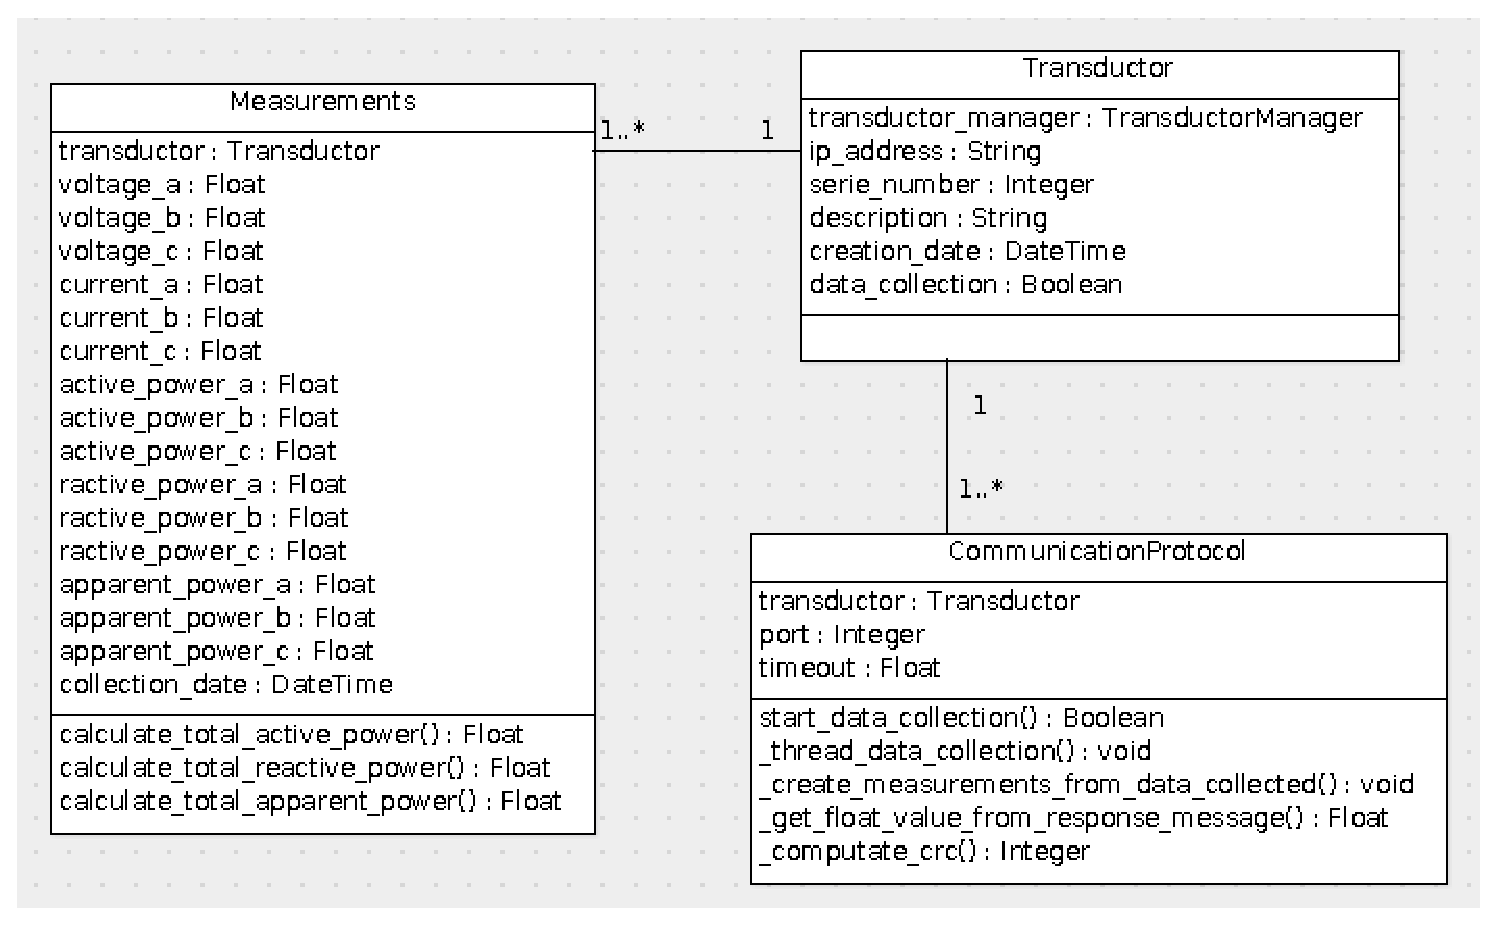
\includegraphics[keepaspectratio=true,scale=0.6]{figuras/sprint01arq.eps}
    \caption{Arquitetura SME-UnB \textit{Sprint 01}. Fonte: autor}
    \label{sprint01arq}
\end{figure}

\vfill
\pagebreak

Foram realizar algumas telas, figuras \ref{dados01} e \ref{dados02}, contendo os dados de energia coletados para apresentação ao usuário.

\begin{figure}[!htpb]
    \centering
    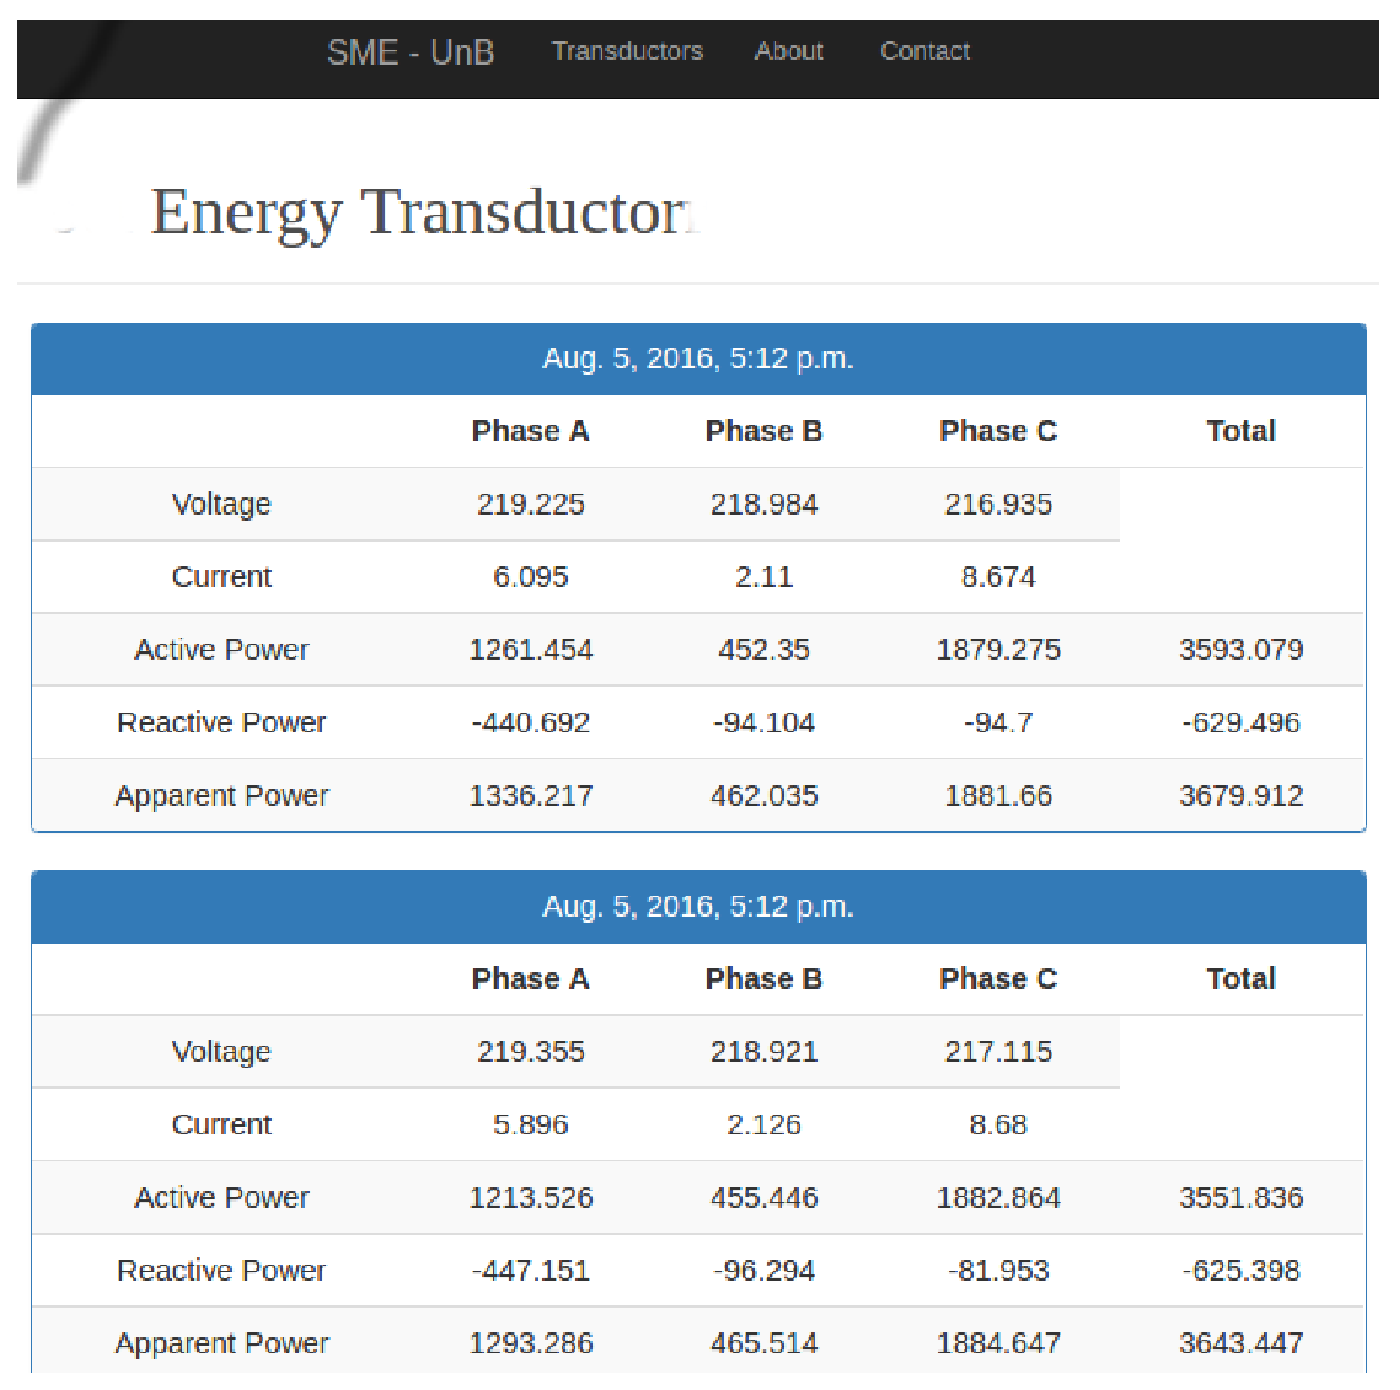
\includegraphics[keepaspectratio=true,scale=0.5]{figuras/coleta_dados_01.eps}
    \caption{Página apresentação medições de energia. Fonte: autor}
    \label{dados01}
\end{figure}

\begin{figure}[!htpb]
    \centering
    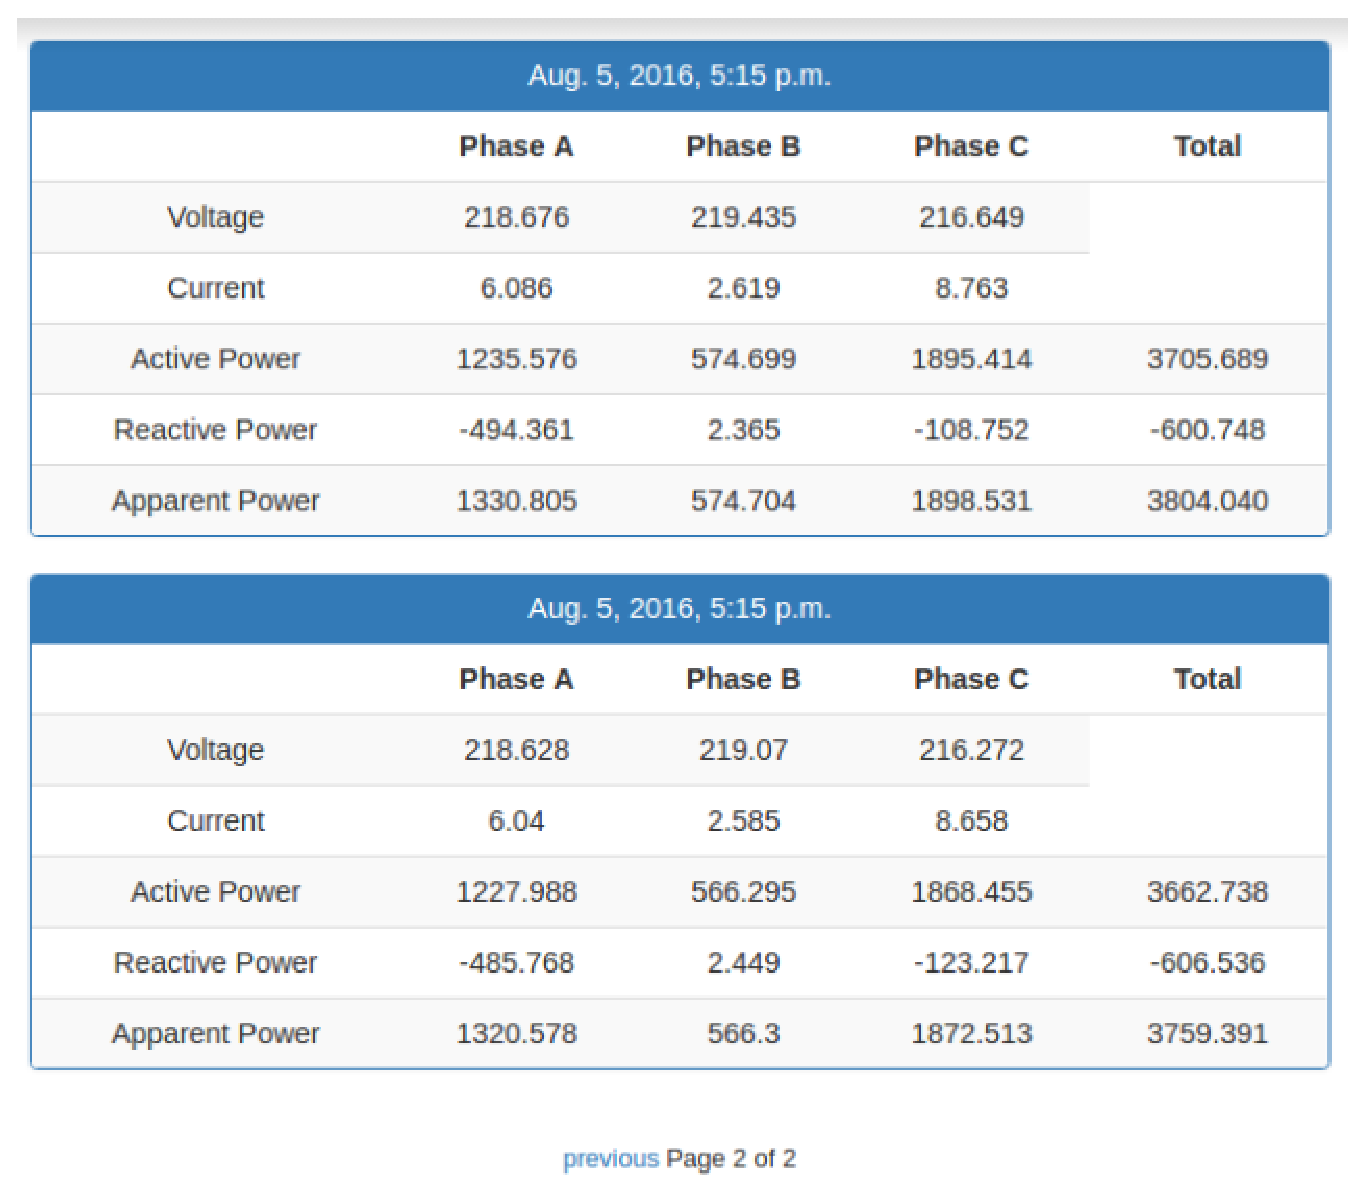
\includegraphics[keepaspectratio=true,scale=0.5]{figuras/coleta_dados_02.eps}
    \caption{Página apresentação medições de energia. Fonte: autor}
    \label{dados02}
\end{figure}

\vfill
\pagebreak

\section{Sprint 02 - Refatorações de Urls/Templates e Guia de Instalação}
Após analisadas as urls e templates do projeto verificou-se que haviam muitas rotas desnecessárias e não havia um padrão para os templates, o que estava gerando confusão na hora de criar novas páginas para a aplicação. Tendo em mente tais problemas essa sprint buscou realizar uma refatoração dos mesmos.

Realizou-se um guia de instalação\footnote{\url{https://gitlab.com/brenddongontijo/SME-UnB/wikis/instalation-guide/}} para o ambiente de desenvolvimento utilizando as ferramentas Vagrant\footnote{\url{https://www.vagrantup.com/}} e Chef Solo\footnote{\url{https://docs.chef.io/chef_solo.html}}, visando auxiliar novos desenvolvedores a contribuirem com o projeto.

\section{Sprint 03}
Realizou-se uma reunião com o orientador visando reestruturar a arquitetura. Primordialmente, tendo em vista que os tradutores podem possuir diferentes tipos de medições, foram definidas duas classes abstratas: Transductor e Measurements. A partir dessas classes surgiram as especializações de transdutores de energia (EnergyTransductor) e medições de energia (EnergyMeasurements). Além disso, percebeu-se a necessidade de criação de um modelo de transdutor (TransductorModel), o qual possuiria informações específicas do mesmo, como endereço e tipo dos registradores, protocolo serial e de transporte utilizados. A figura \ref{sprint03arq} ilustra a evolução da arquitetura realizada nessa sprint.

\begin{figure}[!htpb]
    \centering
    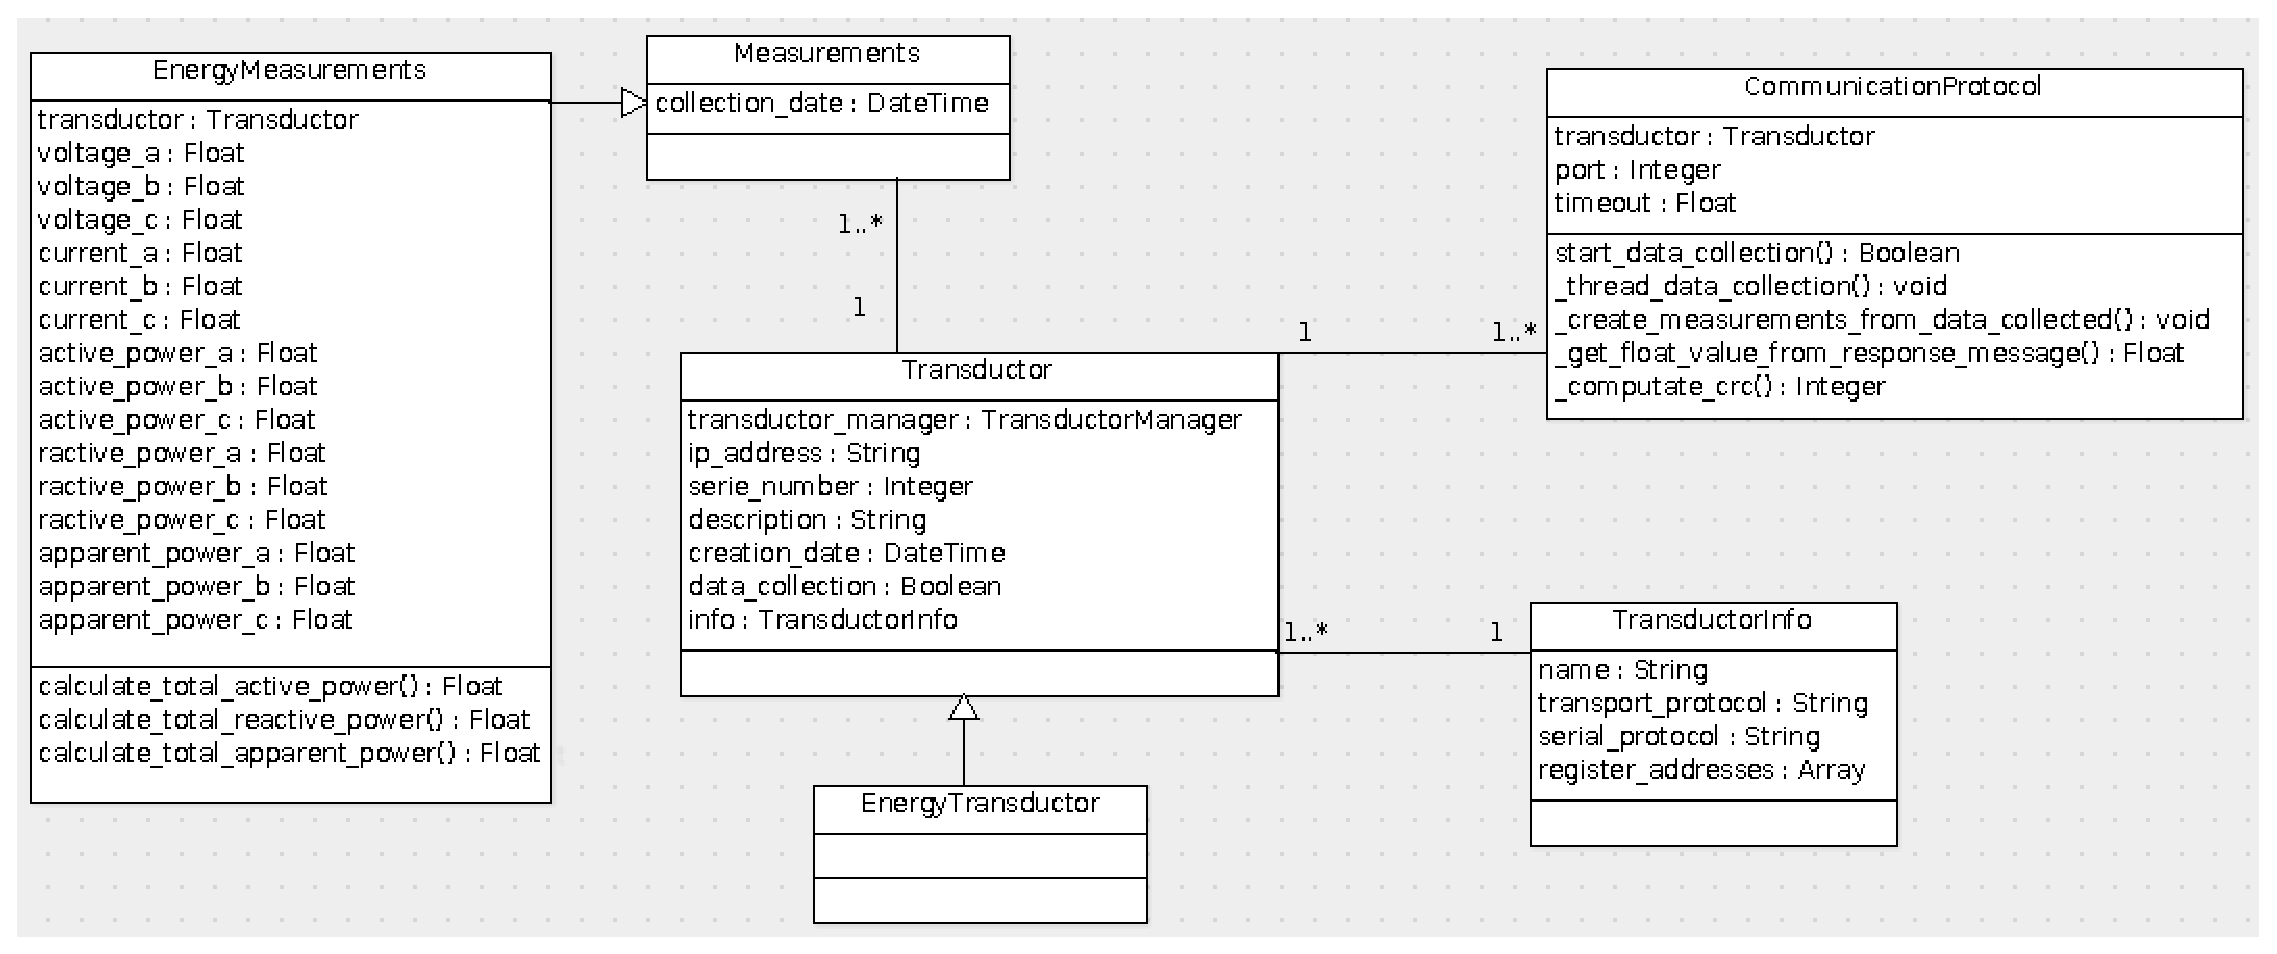
\includegraphics[scale=0.6,angle=90]{figuras/sprint03arq.eps}
    \caption{Arquitetura SME-UnB Sprint 03. Fonte: autor}
    \label{sprint03arq}
\end{figure}

\vfill
\pagebreak

Nessa sprint foi realizado um primeiro contato com os testes e ao seu fim foi obtivo uma cobertura total de 71\%, conforme a figura \ref{cobertura01}.

\begin{figure}[!htpb]
    \centering
    \includegraphics[keepaspectratio=true,scale=0.5]{figuras/cobertura01.eps}
    \caption{Cobertura Total de Código Sprint 03. Fonte: autor}
    \label{cobertura01}
\end{figure}

\section{Sprint 04 - Documentação de Código e Estrutura \textit{Boilerplate}}
Buscando deixar o código mais entendível realizou-se uma documentação geral utilizando os padrões de \textit{docstrings}\footnote{\url{https://www.python.org/dev/peps/pep-0257/}} definidos pelo \textit{Google Python Style}\footnote{\url{http://google.github.io/styleguide/pyguide.html}}. A figura \ref{documentacao01} ilustra um exemplo realizado no projeto.

\begin{figure}[!htpb]
    \centering
    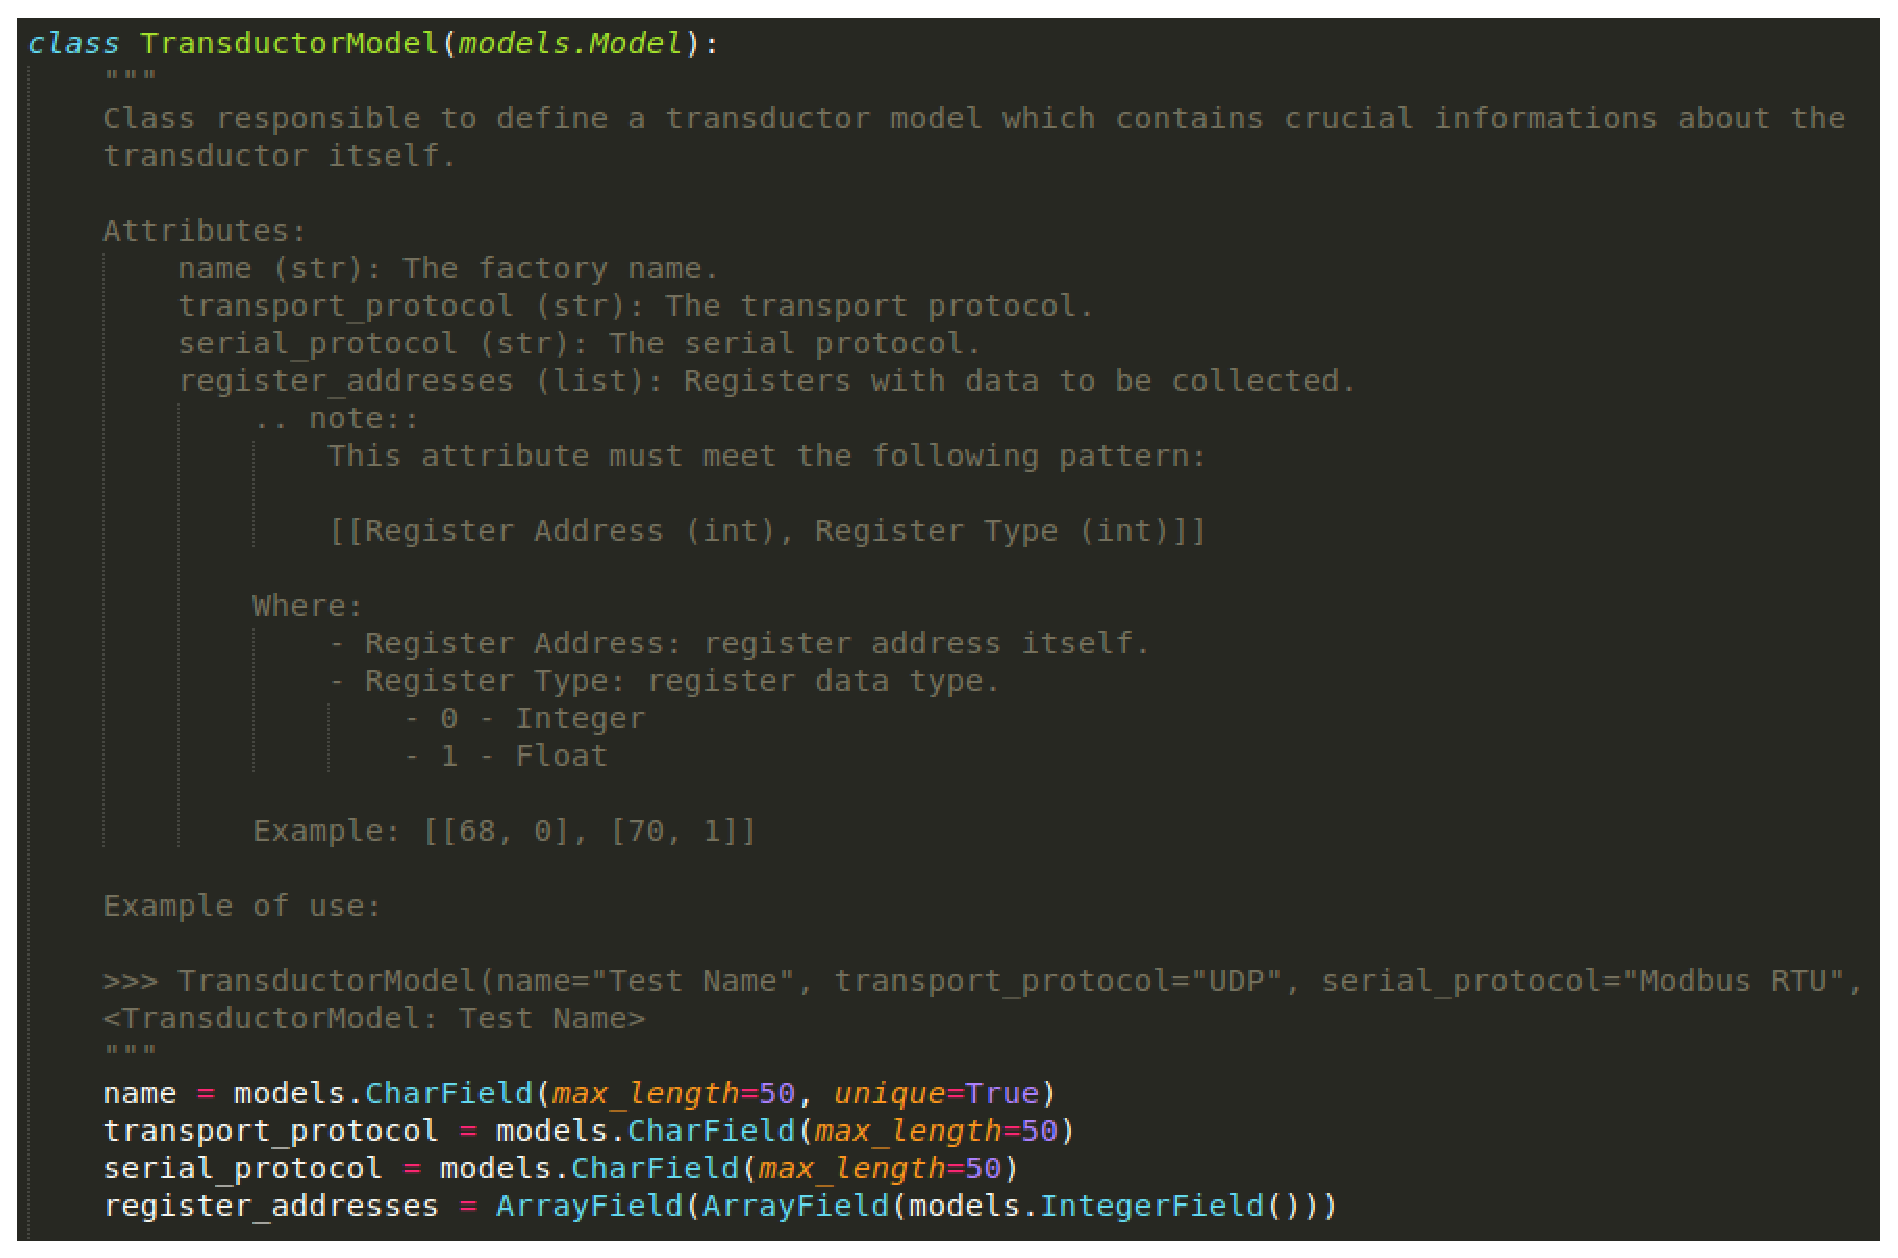
\includegraphics[keepaspectratio=true,scale=0.5]{figuras/documentacao01.eps}
    \caption{Exemplo de Documentação Utilizando \textit{Google Python Style}. Fonte: autor}
    \label{documentacao01}
\end{figure}

A estrutura \textit{Boilerplate}\footnote{\url{https://github.com/fabiommendes/python-boilerplate}} foi adicionada ao projeto com o objetivo de realizar uma melhor estruturação dos módulos e realizar pré-configurações para ambientes de desenvolvimendo/produção, assim como no auxílio para utilização das ferramentas Sphinx e Coverage.

\section{Sprint 05 - Refatoração Arquitetura e Protocolo Serial}
Tendo em vista o forte acoplamento gerado pela classe CommunicationProtocol realizou-se uma mudança na arquitetura, onde a classe em questão foi dividia em duas classes abstratas: TransportProtocol e SerialProtocol. A partir dessas classes foram definidas as especializações referentes ao UdpProtol e ModbusRTU, protocolos os quais são utilizados especificamente pelo modelo de transdutor instalado na Universidade. Além dessas mudanças criou-se uma nova classe chamada EnergyOperations, responsável por realizar cálculos matemáticos com os dados de energia coletados. A figura \ref{sprint05arq} ilustra a evolução arquitetural realizado nessa sprint.
\begin{figure}[!htpb]
    \centering
    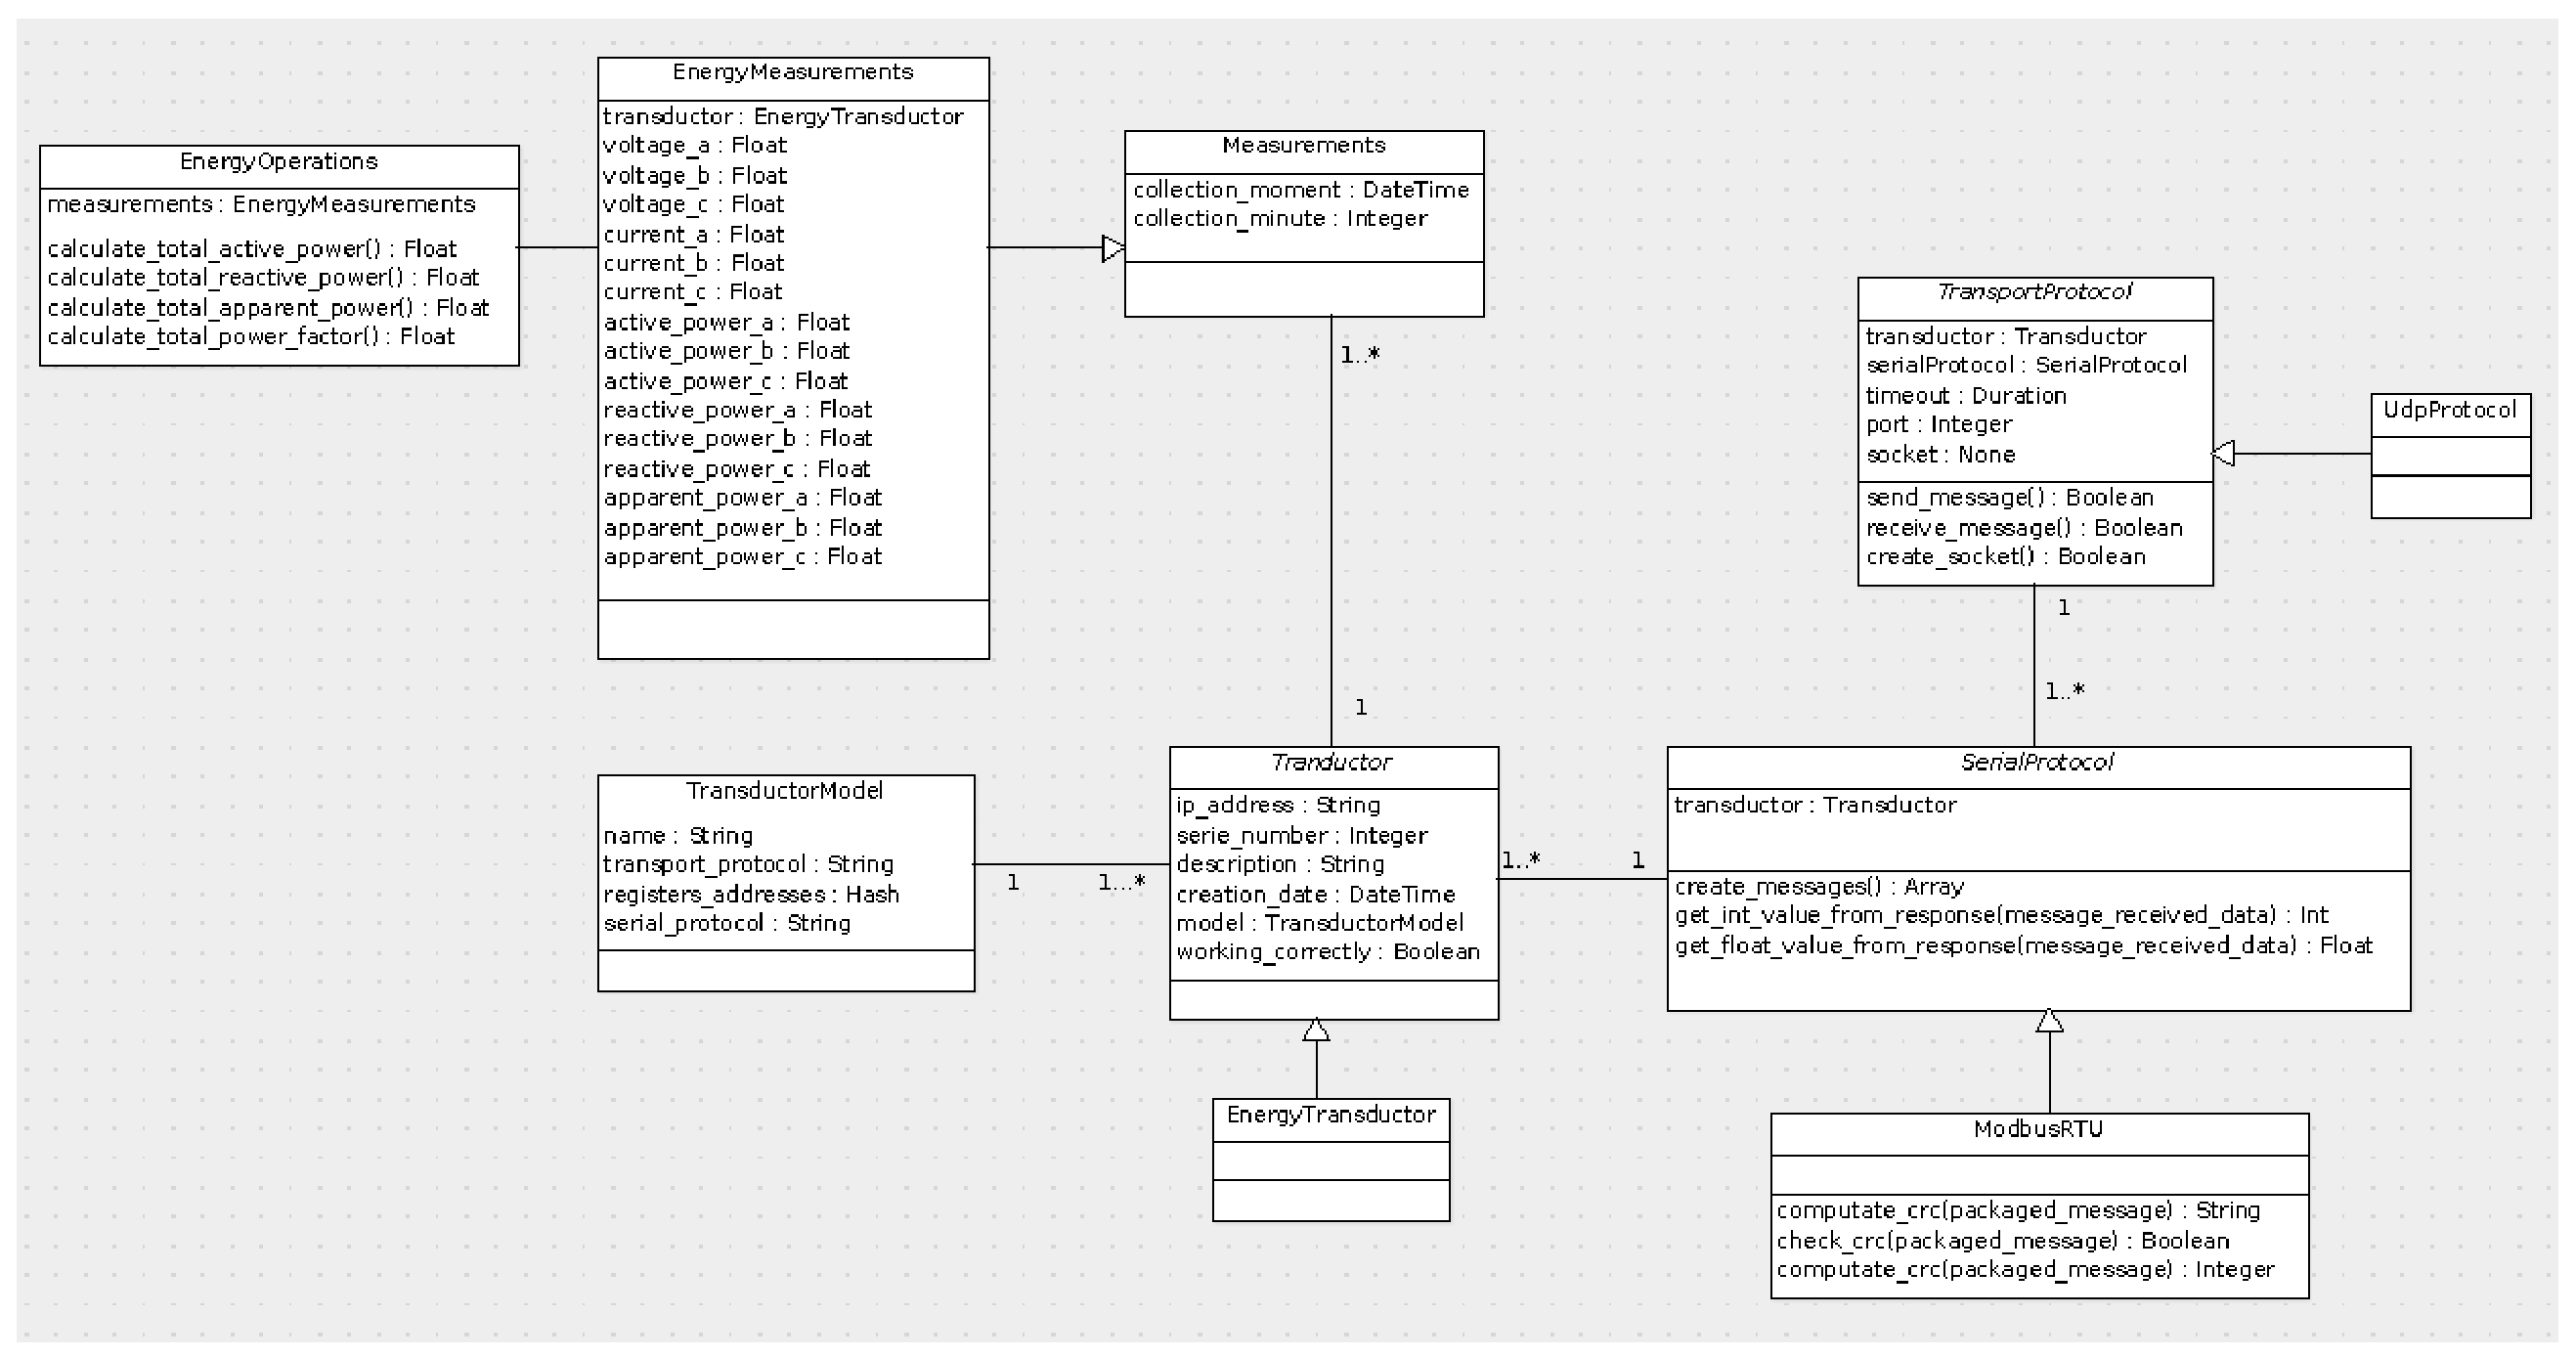
\includegraphics[scale=0.5,angle=90]{figuras/sprint05arq.eps}
    \caption{Arquitetura SME-UnB Sprint 05. Fonte: autor}
    \label{sprint05arq}
\end{figure}

Além das mudanças arquiteturais, foram implementadas e testadas as classes SerialProtocol, ModbusRTU e EnergyOperations. Obteve-se uma cobertura de 96\% ao fim da sprint, conforme ilustrado na figura \ref{cobertura02}.
\begin{figure}[!htpb]
    \centering
    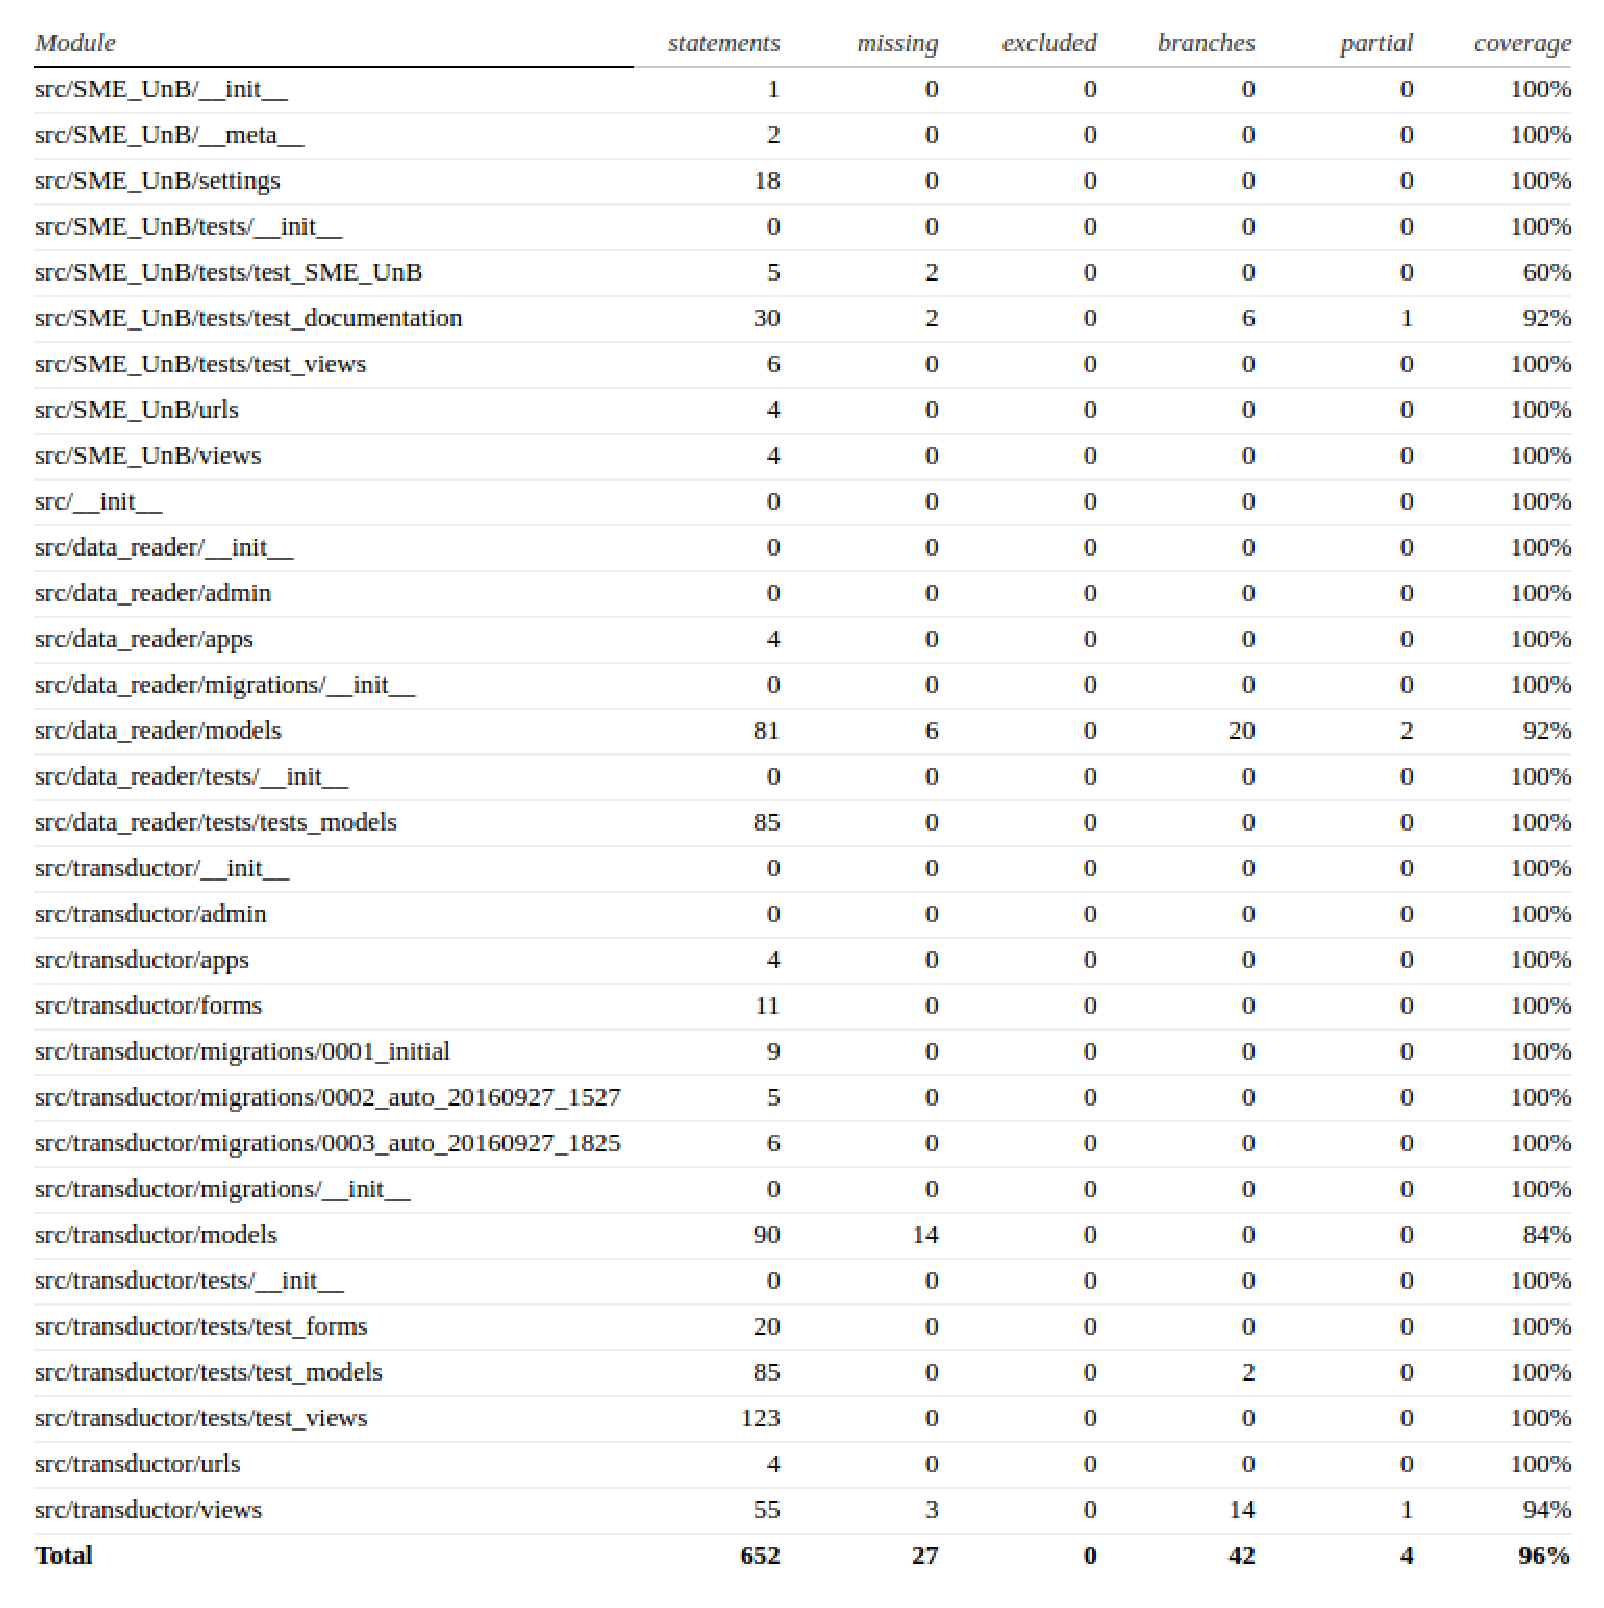
\includegraphics[keepaspectratio=true,scale=0.6]{figuras/cobertura02.eps}
    \caption{Cobertura Total de Código Sprint 05. Fonte: autor}
    \label{cobertura02}
\end{figure}

\section{Sprint 06 - Protocolo de Transporte e Testes com Mock}
Após implementado o protocolo serial, realizou-se o desenvolvimento do protocolo de transporte. Sua principal função é comunicar-se com o transdutor utilizando o protocolo utilizado pelo mesmo e tratar as questões referentes à \textit{timeout} e tentativas consecutivas de envio de requisições. Além disso, foram refatorados os testes do sistema utilizando \textit{Mocks}\footnote{\url{https://docs.python.org/3/library/unittest.mock.html}}, objetivando maior desempenho e efetivamente testar unitariamente os métodos. A figura \ref{exemplo_mock} ilustra um exemplo de teste da classe UdpProtocol utilizando \textit{Mock}. A cobertura de código, figura \ref{cobertura03}, não se alterou comparado à sprint anterior.

\begin{figure}[!htpb]
    \centering
    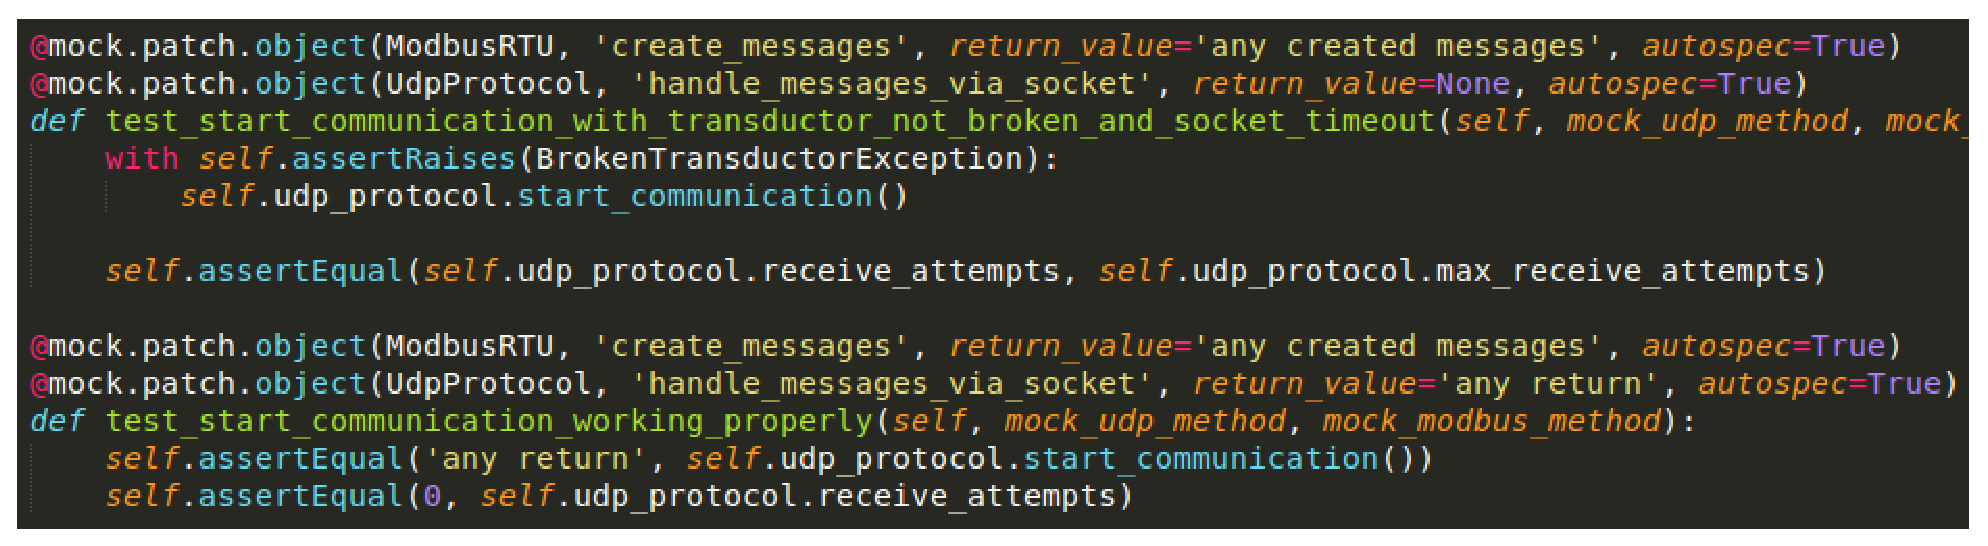
\includegraphics[keepaspectratio=true,scale=0.5]{figuras/exemplo_mock.eps}
    \caption{Exemplo de Teste utilizando \textit{Mock}. Fonte: autor}
    \label{exemplo_mock}
\end{figure}

\begin{figure}[!htpb]
    \centering
    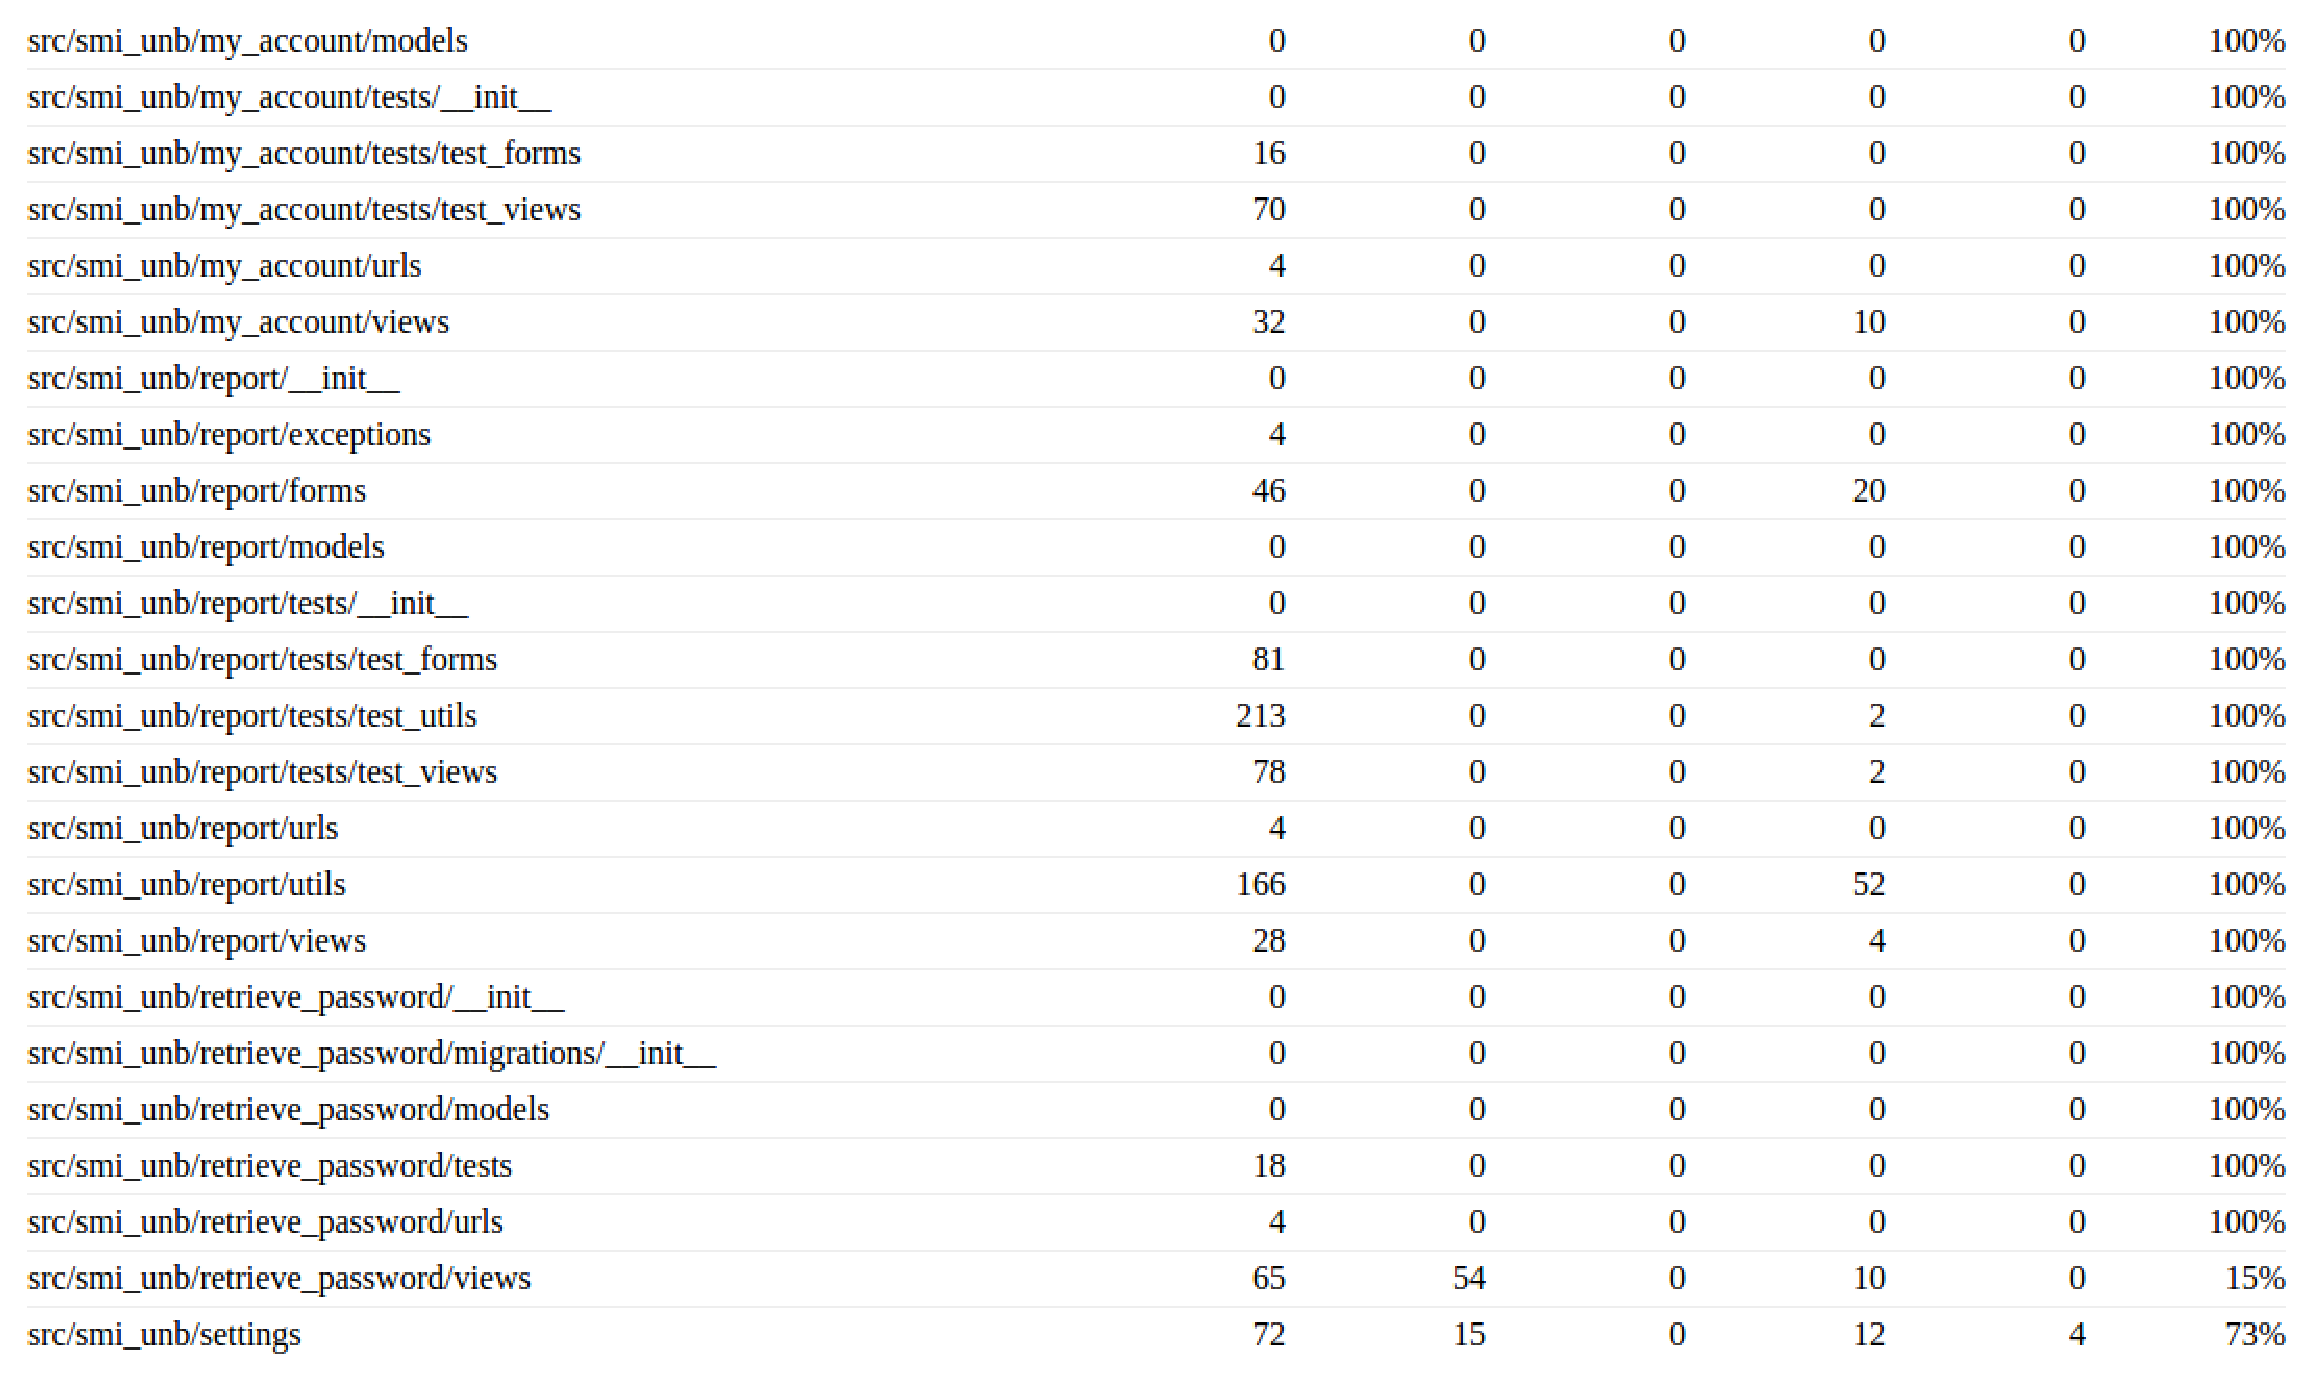
\includegraphics[keepaspectratio=true,scale=0.5]{figuras/cobertura03.eps}
    \caption{Cobertura Total de Código Sprint 06. Fonte: autor}
    \label{cobertura03}
\end{figure}

\section{Sprint 07}

\section{Sprint 08}

\section{Sprint 09}
